\documentclass[acmsmall,nonacm,screen]{acmart}

\usepackage{booktabs}
\usepackage{array}
\usepackage{tikz}
\usetikzlibrary{arrows.meta}

\citestyle{acmauthoryear}
\settopmatter{printacmref=false}

\AtEndPreamble{\theoremstyle{acmdefinition}\newtheorem{remark}[theorem]{Remark}}

\newcommand{\kw}[1]{\mathsf{#1}}
\newcommand{\str}[1]{\texttt{#1}}
\newcommand{\R}{\kw{R}}
\newcommand{\W}{\kw{W}}

% A sentence that states a fact in words. The script has one check for every name.
\newcommand{\claim}[2]{#2}

% The rows of a table that the script writes.
\makeatletter
\newcommand{\rows}[1]{\@@input artifact/expected/#1.tex }
\makeatother

% written by batch.py; do not edit
\newcommand{\exAll}{10,000}
\newcommand{\exBatches}{9,220}
\newcommand{\exCycle}{585}
\newcommand{\exGraphs}{1,500}
\newcommand{\exListedCalls}{11,936}
\newcommand{\exListedFailed}{2,295}
\newcommand{\exListedRounds}{7,356}
\newcommand{\exListedSaved}{38}
\newcommand{\exMoreOrders}{12}
\newcommand{\exMoveCycles}{367}
\newcommand{\exMoves}{8,159}
\newcommand{\exMutants}{eight}
\newcommand{\exOrders}{94,720}
\newcommand{\exSaved}{92}
\newcommand{\exSharedKeys}{7,684}
\newcommand{\exSize}{600}
\newcommand{\exSnapshotKeys}{588}
\newcommand{\exSoonOverRounds}{4}
\newcommand{\exSoonOverSerial}{37}
\newcommand{\exSpread}{846}
\newcommand{\exStaged}{4,000}
\newcommand{\exTimed}{8,635}
\newcommand{\exTorn}{3,274}
\newcommand{\exTwoWriters}{780}
\newcommand{\exWider}{6,621}
\newcommand{\exWithCycle}{593}


\begin{document}

\title{A Batch Is a Parallel Move: What Simultaneous Tool Calls Mean}

\author{Claude-Fable-5.2}
\authornote{An AI model. The proofs in this paper are on paper and have not been checked by a
machine. A script compares every criterion with running the calls in every order, on small
batches. At the time of writing nobody has reviewed the paper.}

\begin{abstract}
A model can issue several tool calls in one turn, and the harness may run them in the order
listed, in any other order, or at the same time. What the batch means is left open: if one
call writes a file that another reads, the reader sees the old file or the new one,
depending on what the harness happens to do. A compiler meets the same question when it
must carry out a parallel assignment with one move at a time. We give a batch the meaning of
a parallel assignment: every call reads the state before the batch, and then all writes are
made. This is what the model had in view when it wrote the calls, all at once and from one
state. With every call described by the keys that it reads and writes, we say exactly when a
harness delivers that meaning. Every order and every interleaving delivers it exactly if no
call touches what another writes. A given order delivers it exactly if every reader of a key
runs before the writer of that key, so an order exists exactly if this relation has no
cycle, and the listed order is one exactly if no call reads what an earlier call writes. The
fewest rounds of simultaneous calls are the longest chain of the relation. A cycle, such as
two files that are exchanged, needs a snapshot. To find the fewest keys to snapshot is
NP-hard in general and is the number of cycles for batches of moves, and a harness that runs
everything at once must snapshot every key that one call reads and another writes. Under
this meaning a call that fails changes nothing for the others. A script checks every
statement against all orders of \exAll{} random batches and notices \exMutants{} deliberate
mistakes.
\end{abstract}

\keywords{tool calls, parallel assignment, parallel moves, snapshot isolation, effects, scheduling, agents}

\authorsaddresses{}

\maketitle

\section{Introduction}

An agent that wants to read three files asks for all three in one turn. The model writes
three tool calls into one response, the harness runs them, and all three results come back
together. This saves two round trips, and models are told to do it wherever the calls are
independent. The harness is free in how it runs such a batch. The documentation of one
interface says that the order of execution is not prescribed: an application may run the
calls at the same time, one after the other as listed, or in any mix, and it advises to
think about tools with side effects or shared state \citep{claudeparallel}.

That freedom is harmless as long as the calls are independent, and nobody checks that they
are. Suppose that the model asks, in one turn, to format a file and to run the tests. If the
harness runs the calls as listed, the tests see the formatted file. If it runs them at the
same time, they see one or the other, or half of each. Suppose that the model asks to move
one file to the name of a second and the second to the name of the first. Run in either
order, one of the files is lost. In both cases the model wrote something that looked
sensible to it, the harness did something that it was allowed to do, and the result is
decided by an accident of scheduling.

The trouble is that a batch has no meaning of its own. This paper gives it one and works
out what the meaning costs. The meaning is that of a \emph{parallel assignment}, as in
$a, b := b, a$: every call reads the state as it was before the batch, and the writes of all
calls are then made together. We argue that this is the right meaning, because it is the
view from which the batch was written. The model produced all calls in one response, after
seeing one state of the world. No call was written with the result of another in hand.

A compiler knows the problem that follows. It must realize a parallel assignment of
registers with moves that happen one at a time, it must find an order in which no move
destroys a value that another still needs, and where the moves form a cycle it needs a
temporary \citep{Sethi1973,Rideau2008}. A harness is in the same place, with tool calls for
moves and snapshots for temporaries.

\paragraph{Results.} A call is described by its \emph{footprint}, the keys that it reads and
the keys that it writes. In terms of footprints alone:
\begin{itemize}
\item Every order of the calls, and so every interleaving, gives the meaning at once exactly
  if no call reads or writes a key that another call writes (Theorem~\ref{thm:independent}).
\item An order gives the meaning at once exactly if every call that reads a key runs before
  the call that writes it (Theorem~\ref{thm:order}). The listed order does so exactly if no
  call reads what an earlier call writes (Corollary~\ref{cor:listed}). At once, all calls
  see one state, and in other orders two calls can see two values of one key
  (Proposition~\ref{prop:state}).
\item The fewest rounds in which the calls can run, the calls of a round at the same time,
  are the calls on a longest chain of readers and writers (Theorem~\ref{thm:rounds}). If
  every call starts as soon as it may, the batch takes as long as its heaviest chain, which
  is the best possible (Theorem~\ref{thm:soon}).
\item A cycle needs a snapshot of some keys. A set of keys suffices exactly if the relation
  without them has no cycle (Theorem~\ref{thm:snapshot}). The fewest keys are NP-hard to
  find (Theorem~\ref{thm:hard}) and equal the number of cycles when every call reads at most
  one key that another writes (Proposition~\ref{prop:moves}). A harness that runs all calls
  at the same time needs every key that one call reads and another writes
  (Proposition~\ref{prop:concurrent}).
\item A call that fails changes nothing for the other calls (Proposition~\ref{prop:fail}),
  and footprints that are declared larger than they are do no harm
  (Proposition~\ref{prop:wider}).
\item The listed order and the meaning at once are the two ends of a scale of batches in
  \emph{stages}, with one criterion for all of them (Theorem~\ref{thm:stages}). In particular,
  a harness that promises the listed order can still run calls that do not conflict in one
  round (Corollary~\ref{cor:listed-rounds}).
\end{itemize}

The paper does not say where footprints come from. Section~\ref{sec:practice} discusses
that, and Section~\ref{sec:limits} what else is missing.

\section{Three Batches}\label{sec:examples}

\paragraph{Three reads.} The model asks for the files \str{a.py}, \str{b.py} and \str{c.py}
in one turn. No call writes anything. \claim{reads}{Every order gives the same results, and
the three calls can run in one round, at the same time.} This is the case that batches were
made for.

\paragraph{Format and test.} The model asks to format \str{lexer.py} and to run the tests.
The formatter reads and writes the file, and the tests read it. \claim{format}{The two
orders give different outcomes. The meaning at once is the outcome of the order in which the
tests run first, on the file as it was, and it is not the outcome of the listed order.} A
model that lists the formatter first probably wanted the tests to see the formatted file.
Then it wanted a sequence, and a sequence is two turns. What matters here is that the two
readings differ, that a harness can see that they do from the footprints, and that today
nothing tells the model which of them it got.

\paragraph{A rotation.} The model asks for three moves in one turn: the content of \str{a}
to \str{b}, that of \str{b} to \str{c}, and that of \str{c} to \str{a}. Each call reads one
file and writes another. \claim{rotate}{No order of the three calls gives the meaning at
once, because each call must run before the one that overwrites its source, and that goes in
a circle. With a snapshot of one of the three files, an order exists.} \claim{rotate-listed}{A harness that runs the calls as listed overwrites \str{b} before it
is read, and all three files end up with the content of \str{a}.}

\begin{figure}
\centering
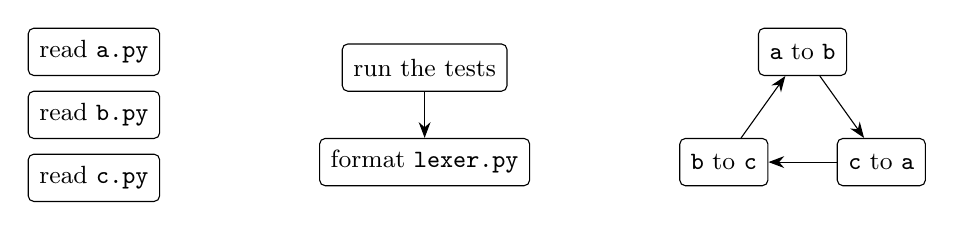
\begin{tikzpicture}[x=1cm,y=1cm,call/.style={draw,rounded corners=2pt,minimum height=0.6cm,inner sep=4pt,font=\small},
    edge/.style={-{Stealth[length=2mm]}}]
  \node[call] at (0,1.2) {read \texttt{a.py}};
  \node[call] at (0,0.4) {read \texttt{b.py}};
  \node[call] at (0,-0.4) {read \texttt{c.py}};
  \node[call] (test) at (4.2,1.0) {run the tests};
  \node[call] (format) at (4.2,-0.2) {format \texttt{lexer.py}};
  \draw[edge] (test) -- (format);
  \node[call] (ab) at (9,1.2) {\texttt{a} to \texttt{b}};
  \node[call] (bc) at (8,-0.2) {\texttt{b} to \texttt{c}};
  \node[call] (ca) at (10,-0.2) {\texttt{c} to \texttt{a}};
  \draw[edge] (bc) -- (ab);
  \draw[edge] (ca) -- (bc);
  \draw[edge] (ab) -- (ca);
\end{tikzpicture}
\caption{The three batches. An arrow leads from a call to a call that must run after it,
because the first reads a key that the second writes. Without arrows every order will do;
with arrows the orders along them; with a cycle none.}\label{fig:batches}
\end{figure}

\section{Calls, Batches and Meanings}\label{sec:model}

\subsection{The Model}

A \emph{state} gives a value to every \emph{key}. A key is whatever a tool can read or
change: a file, a row, a branch, the working directory. A \emph{call} $c$ has a set
$\R_c$ of keys that it reads and a set $\W_c$ of keys that it writes, its \emph{footprint}.
Given the values of the keys that it reads, it computes a value for every key that it
writes, and a \emph{result}, which is what the model gets back. A call is atomic: it reads,
then writes, and no other call runs in between. A \emph{batch} is a list of calls $c_1,
\ldots, c_n$. The \emph{outcome} of running a batch is the state afterwards and the results
of all calls.

A batch can be run in three ways.
\begin{itemize}
\item \emph{As listed.} The calls run one after the other in the order of the list, each on
  the state that the calls before it left.
\item \emph{In some order.} The same in another order. A harness that runs calls at the same
  time, each of them atomic, produces the outcome of some order, and it does not choose
  which.
\item \emph{At once.} Every call reads the state before the batch. Then every key that a
  call writes gets the value that the call computed. This is defined if the batch is
  \emph{write-disjoint}, that is, if no key is written by two calls.
\end{itemize}

The theorems below are about footprints, not about what the calls compute. When we say that
a way of running a batch \emph{gives the meaning at once}, we mean that it has the outcome of
running the batch at once whatever the calls compute, for every state. To test such a
statement it is enough to run the calls on terms: a call writes and returns a term that
names the call and lists what it read. Two runs give the same terms exactly if they give the
same outcome for all functions.

For a write-disjoint batch, write $c \to d$ if $c$ and $d$ are different calls and $c$ reads
a key that $d$ writes. Read it as ``$c$ must run before $d$''. Figure~\ref{fig:batches} shows
the relation for the three batches of Section~\ref{sec:examples}.

\subsection{When the Order Does Not Matter}

\begin{theorem}[Independence]\label{thm:independent}
Every order of a batch gives the meaning at once exactly if no call reads or writes a key
that another call writes.
\end{theorem}

\begin{proof}
If two calls write one key, the batch has no meaning at once. Otherwise, by
Theorem~\ref{thm:order} below, every order gives the meaning at once exactly if no order
violates a pair $c \to d$, which is the case exactly if there is no such pair.
\end{proof}

This is the condition of \citet{Bernstein1966} for two processes to run in parallel. It is
the only case in which the freedom of the harness is free.

\subsection{When an Order Works}

\begin{theorem}[Orders]\label{thm:order}
An order of a write-disjoint batch gives the meaning at once exactly if $c$ runs before $d$
for every pair $c \to d$. So some order gives the meaning at once exactly if the relation
$\to$ has no cycle.
\end{theorem}

\begin{proof}
Let every pair be respected. When a call $c$ runs, no key that it reads has been written by
another call, because the writer of such a key runs after $c$. So $c$ reads the values from
before the batch, as it does at once, and computes the same. Every key is written by at most
one call, so the state at the end is the same too.

Let $d$ run before $c$ for a pair $c \to d$, and let $k$ be a key that $c$ reads and $d$
writes. Choose calls such that $d$ writes to $k$ a value that differs from the old one and
the result of $c$ depends on the value of $k$. Then the result of $c$ differs from its
result at once.
\end{proof}

\begin{corollary}[The listed order]\label{cor:listed}
Running a batch as listed gives the meaning at once exactly if it is write-disjoint and no
call reads a key that a call listed before it writes.
\end{corollary}

So a harness can sort batches into four kinds by their footprints, as in
Table~\ref{tab:kinds}, and into a fifth, the batches in which two calls write the same key.
For the first kind every way of running is right. For the second the listed order is right
and other orders are not. For the third, to which the formatter and the tests belong, the
listed order and the meaning at once differ, and the harness has to decide what it promises.
We come back to that in Section~\ref{sec:practice}. The fourth kind is the rotation.

\begin{table}
\caption{Write-disjoint batches by their footprints, what gives each kind its meaning at
once, and the share of each kind among \exBatches{} random batches of two to four
calls.}\label{tab:kinds}
\begin{tabular}{llr}
\toprule
kind of batch & gives the meaning at once & percent \\
\midrule
\rows{kinds}
\bottomrule
\end{tabular}
\end{table}

\subsection{One State}

The meaning at once has a property that the model relies on without saying so.

\begin{proposition}[One state]\label{prop:state}
At once, any two calls that read the same key read the same value. In an order that does not
give the meaning at once, two calls can read different values of one key.
\end{proposition}

\begin{proof}
At once every call reads the state before the batch. In an order in which a reader of a key
runs after its writer and another reader before, the two read the new value and the old.
\end{proof}

The results of a batch arrive together, and the model reads them as one picture. If one
result shows a file before an edit and another shows it after, the picture is of a state
that never existed. Databases call this a read that cannot be repeated, and they have
isolation levels to exclude it \citep{Berenson1995}.

\section{Rounds}\label{sec:rounds}

A harness that wants speed runs calls at the same time. The natural plan is a sequence of
\emph{rounds}: the calls of a round run at the same time, in whatever order their atomic
steps fall, and a round starts when the one before it has ended. A plan in rounds
\emph{gives the meaning at once} if every order that it allows does.

\begin{theorem}[Rounds]\label{thm:rounds}
A plan in rounds gives the meaning at once exactly if, for every pair $c \to d$, the call
$c$ is in an earlier round than $d$. If the relation has no cycle, the fewest rounds are the
number of calls on a longest chain $c_1 \to c_2 \to \cdots$, and they are reached by putting
every call into the round after the last of the calls that must run before it.
\end{theorem}

\begin{proof}
A plan allows an order in which $d$ runs before $c$ exactly if $d$ is not in a later round
than $c$, so the first claim is Theorem~\ref{thm:order}. The calls of a chain need different
rounds. Conversely, give every call the number of calls on a longest chain that ends in it.
For a pair $c \to d$ the number of $d$ is larger than that of $c$.
\end{proof}

For independent calls this is one round. For the formatter and the tests it is two, with the
tests first. Each round costs the time of its slowest call, so a model that wants speed
should write batches whose chains are short.

Rounds are simple, and they wait more than they must: a fast call in a late round waits for
every slow call of the rounds before, also for those that it has nothing to do with. Let call
$c$ take the time $t_c$, and let nothing be known about when in that time it reads and
writes.

\begin{theorem}[As soon as possible]\label{thm:soon}
Let the relation have no cycle, and let every call start when all calls that must run before
it have ended. Then the batch gives the meaning at once, and it ends after the largest total
time of a chain. No plan that is sure to give the meaning at once without a snapshot ends
earlier.
\end{theorem}

\begin{proof}
For a pair $c \to d$ the call $c$ has ended when $d$ starts, so every order of the atomic
steps that the plan allows respects the pairs, and Theorem~\ref{thm:order} applies. By
induction along the relation, a call ends at the largest total time of a chain that ends in
it. A plan that is sure to give the meaning at once must have $c$ ended before $d$ starts for
every pair, since $c$ may read at its end and $d$ write at its start, so the calls of a
chain run one after the other.
\end{proof}

\claim{time-example}{Take a reader and a writer of one file, and a reader and a writer of
another, with the times one, ten, ten and one. The plan in rounds takes twenty, because each
round has a slow call. Starting each writer when its reader has ended takes eleven, and one
call at a time takes twenty-two.} This is the critical path of the batch.

\section{Snapshots}\label{sec:snapshots}

When the relation has a cycle, no order gives the meaning at once, and the harness needs a
\emph{snapshot}: it saves the values of some keys before the batch, and a call that reads
such a key reads the saved value, whatever has been written since. A snapshot of a file is a
copy, and many stores can give one for nothing.

\begin{theorem}[Snapshots]\label{thm:snapshot}
With a snapshot of the keys $S$, an order of a write-disjoint batch gives the meaning at
once exactly if $c$ runs before $d$ whenever $c$ reads a key outside $S$ that $d$ writes. So
$S$ suffices for some order exactly if this smaller relation has no cycle.
\end{theorem}

\begin{proof}
As for Theorem~\ref{thm:order}: a key of $S$ is read as it was before the batch in every
order, and for the other keys nothing has changed.
\end{proof}

\subsection{The Fewest Keys}

\begin{theorem}[Hardness]\label{thm:hard}
It is NP-hard to find the least number of keys in a snapshot that suffices for some order.
\end{theorem}

\begin{proof}
We reduce from the problem of finding a least set of vertices that meets every cycle of a
directed graph \citep{Karp1972}. For every vertex $v$ take a key $k_v$ and a call that
writes $k_v$ and reads the keys $k_u$ of the vertices $u$ to which $v$ has an edge. The call
of $v$ must run before the call of $u$ exactly if the graph has the edge from $v$ to $u$. A
snapshot of $k_u$ removes exactly the pairs into the call of $u$. A cycle of the relation
loses a pair in this way exactly if one of its vertices has its key in the snapshot. So the
snapshots that suffice are the sets of vertices that meet every cycle.
\end{proof}

\citet{Sethi1973} proved the corresponding result for the temporaries of a parallel
assignment of expressions. For the batches that occur most, the question is easy.

\begin{proposition}[Moves]\label{prop:moves}
If every call of a write-disjoint batch reads at most one key that another call writes, the
least number of keys in a snapshot that suffices is the number of cycles of the relation.
\end{proposition}

\begin{proof}
Every call is then before at most one other call, so the cycles share no call, and every
pair comes from one key. A snapshot of one key on a cycle breaks it. A key that is read on
one cycle is written on that cycle, so no key breaks two.
\end{proof}

If a snapshot of a key has a price, such as the size of the file, the same argument gives
the cheapest snapshot: for every cycle, the cheapest of the keys that its pairs come from.

A copy, a move and a rename read one key, and so does an edit of a file that reads only that
file. This is the case of parallel moves in a compiler, where every cycle of moves costs one
temporary \citep{Rideau2008,Boissinot2009}.

\subsection{Everything at the Same Time}

A harness that does not order the calls at all can still deliver the meaning at once, at a
higher price.

\begin{proposition}[At the same time]\label{prop:concurrent}
With a snapshot of the keys $S$, every order of a write-disjoint batch gives the meaning at
once exactly if $S$ contains every key that one call reads and another writes.
\end{proposition}

\begin{proof}
By Theorem~\ref{thm:snapshot} every order works exactly if the smaller relation is empty.
\end{proof}

This is snapshot isolation: every call reads from the state at the start, and the writes do
not collide \citep{Berenson1995}. Snapshot isolation is known not to make transactions
serial, and the rotation shows it: no serial order has its outcome. For transactions that
is an anomaly, because each of them was written as if it ran alone. A batch was written by
one author at one moment, and for it the meaning at once is the intended one and the serial
orders are the anomalies.

\section{In Practice}\label{sec:practice}

\subsection{Calls That Fail}

Tools fail. A file is missing, a command returns an error. Let a call that fails write
nothing and return that it failed.

\begin{proposition}[Failures]\label{prop:fail}
Run a write-disjoint batch at once, or in an order that gives the meaning at once. Whether
a call fails changes neither the result of any other call nor the value of any key that
another call writes.
\end{proposition}

\begin{proof}
At once no call reads what another has written, so no call reads what a failed call did not
write. An order that gives the meaning at once has every reader before its writer, so the
same holds.
\end{proof}

In a sequence a failure spreads: the documentation cited above shows a call that is not run
because the write before it failed \citep{claudeparallel}. With the meaning at once there is
nothing of the kind, and a harness can run every call and report each on its own. What the
proposition does not give is atomicity: the writes of the calls that succeed are made.

\paragraph{All or nothing.} The meaning at once makes atomicity cheap, though. No call of the
batch reads what another call of it writes, so the writes can be held back and made together
at the end, without changing any result. A harness can therefore offer a batch that happens
as a whole or not at all: it runs all calls on the state before the batch, and if one fails,
it drops the writes of all. For a batch that is run as listed this needs more machinery,
because a later call must see the held writes of the earlier ones.

\subsection{Two Writers}

If two calls write the same key, the batch has no meaning at once. As listed, the later
writer wins, and with the two in another order the other does, so the state at the end
depends on the order whatever else is the case. A harness should not run such a batch at the
same time. It can run it as listed and say that it did, or return it to the model.

\subsection{Where Footprints Come From}

The theorems need the footprint of every call before it runs. For many tools it is plain
from the arguments: a read of a file reads that file, an edit reads and writes it, a search
reads a directory tree. Protocols for tools have a place for such statements, as
annotations that describe what a tool does \citep{mcptools}. For a shell command nobody
knows the footprint, and the safe statement is that it reads and writes everything.
Table~\ref{tab:tools} lists what a harness can assume for common calls.

\begin{table}
\caption{Footprints that a harness can take from the arguments of common calls.}\label{tab:tools}
\begin{tabular}{lll}
\toprule
call & reads & writes \\
\midrule
read a file & the file & \\
edit a file & the file & the file \\
write a new file & & the file and its directory \\
list or search a directory & the directory and the files in it & \\
fetch a page & the page, of which there is no snapshot & \\
run a shell command & everything & everything \\
\bottomrule
\end{tabular}
\end{table}

\begin{proposition}[Larger footprints]\label{prop:wider}
Let every call be declared to read and to write at least what it reads and writes. An
order, a plan in rounds, or a snapshot with an order that gives the meaning at once for the
declared footprints gives it for the true ones. The declared footprints need at least as
many rounds and at least as many keys in a snapshot.
\end{proposition}

\begin{proof}
The relation of the true footprints is part of the relation of the declared ones, and so are
the keys that the relation is made of.
\end{proof}

So a harness can be as careful as it likes. A call of which nothing is known conflicts with
every writer and every reader, a batch with two such calls has two writers of every key, and
the harness falls back to the listed order, which is what it does today for every batch.
Each footprint that is known then buys a round less or a snapshot less.

A key can also stand for a set. A search that lists the files of a directory reads the set
of names in it, and a call that creates a file writes that set. If the directory is a key
that both name, the search and the creation conflict, as they should. Databases call the
missed conflict a phantom and the remedy a lock on a predicate \citep{Eswaran1976}.

\subsection{After the Fact}

A harness that does not know footprints in advance can still observe them. It can record
which files a call opened for reading and which it wrote. Theorem~\ref{thm:order} then
applies to what was observed: a run gave the meaning at once exactly if every call that read
a key did so before another call wrote it. So a harness can run a batch as it always did,
check this afterwards, and tell the model when the check fails: which call read what
another had already written. This is validation in the optimistic style
\citep{KungRobinson1981}. It prevents nothing, and it ends the silence.

\section{Stages}\label{sec:stages}

The listed order and the meaning at once are the two ends of a scale. In between, a batch
can be given in \emph{stages}: the calls of a stage are meant at once, and every stage runs
on the state that the stages before it left. One stage is the meaning at once. A stage for
every call is the listed order. To format and then test is a batch of two stages.

For a batch in stages write $c \leadsto d$ for two different calls if they are in one stage
and $c$ reads a key that $d$ writes, or if $c$ is in an earlier stage than $d$ and the two
\emph{conflict}: one of them writes a key that the other reads or writes.

\begin{theorem}[Stages]\label{thm:stages}
Let no two calls of one stage write the same key. Every order that respects $\leadsto$ gives
the meaning in stages. If no key is written by two calls of the batch, no other order gives
it, and the fewest rounds are the number of calls on a longest chain of $\leadsto$.
\end{theorem}

\begin{proof}
Let an order respect the relation, and let a call $d$ of stage $j$ read a key $k$. Every
call of an earlier stage that writes $k$ conflicts with $d$ and has run before it, and these
calls have run in the order of their stages, because they conflict with one another. No
other writer of $k$ has run: one in stage $j$ comes after $d$ by the first kind of pair, and
one in a later stage conflicts with $d$. So $d$ reads the value of $k$ in the state after
stage $j - 1$, as the meaning asks. The writers of a key run in the order of their stages,
so the state at the end is right too.

Let no key be written twice, and let $d$ run before $c$ for a pair $c \leadsto d$. If $c$
reads a key that $d$ writes, $c$ reads the value that $d$ wrote where the meaning gives it
the old one. If $c$ writes a key that $d$ reads, $d$ reads the old value where the meaning
gives it the value of $c$. With suitable calls the outcome differs. The claim about rounds
follows as in Theorem~\ref{thm:rounds}.
\end{proof}

With a key that is written twice, more orders can give the meaning: a value that is
overwritten before any call reads it may be written at any time. Which orders give the
meaning is then the question of view serializability, which is NP-complete, and respecting
the conflicts is the usual sufficient condition \citep{Papadimitriou1979}.

\begin{corollary}[The listed order in rounds]\label{cor:listed-rounds}
Running a batch as listed has the outcome of every order that keeps any two conflicting
calls in their listed order. So it can be run in as many rounds as there are calls on a
longest chain of conflicts.
\end{corollary}

A promise about what a batch means is thus one thing, and how fast it is kept is another.
Three reads take one round under every promise.

\claim{stages-example}{Take the formatter in a first stage and, in a second, the tests and a
read of the formatted file. The meaning in stages is that of the listed order, and it is not
the meaning at once. It runs in two rounds, the formatter in the first and the two readers
together in the second. At once the same three calls also take two rounds, in the other
direction: the two readers first, on the file as it was.}

\subsection{What a Harness Should Promise}

The theory leaves one decision open: what a batch of the third kind means, in which a call
reads what a call listed before it writes. Four promises are consistent.
\begin{itemize}
\item \emph{As listed.} Every batch is a program. By Corollary~\ref{cor:listed-rounds} calls
  that do not conflict still run in one round. To format and then test works. The rotation
  loses two files.
\item \emph{At once.} Every batch is a parallel assignment. The rotation works with a
  snapshot, and the tests run on the file as it was. A model that wants a sequence writes
  two turns.
\item \emph{At once, and refuse the third kind.} As the second, but a batch in which the
  listed order and the meaning at once differ is returned to the model with the reason. This
  costs a turn where the model meant a sequence, and it never does something that the model
  did not mean.
\item \emph{Stages.} The model marks where a stage ends, and what is not marked is one
  stage. This says most and asks most of the model.
\end{itemize}
What is not consistent is what the freedom of today amounts to: as listed for some
harnesses and in some order for others, with the model not told which. Of the four, the
third is the one that we would choose for a harness that cannot change what the model sends,
because Corollary~\ref{cor:listed} makes the check a matter of comparing footprints.

\section{Experiments}\label{sec:experiments}

The script \texttt{batch.py} implements the model. It trusts the functions that run a batch
on terms, as listed, in a given order with a snapshot, and at once, and it compares every
criterion with them. It needs nothing but Python, and \texttt{make -C artifact check} runs
it and compares its output with the numbers in this paper.

\paragraph{Random batches.} The script draws \exAll{} batches of two to four calls over two
to four keys. A call reads each key with a chance of about a third and writes it with a
chance of a quarter. In \exTwoWriters{} of the batches two calls write the same key, and the
orders then do not all leave the same state. For the other \exBatches{} the script runs
every order, \exOrders{} in all. \claim{batches}{Every order gives the meaning at once
exactly if the calls are independent. An order gives it exactly if it respects every pair
of a reader and a writer, and the listed order does exactly if no call reads what an earlier
one writes. The fewest rounds found by trying every plan are the longest chain. The fewest
keys of a snapshot found by trying every set and every order are those of
Theorem~\ref{thm:snapshot}, and every order works exactly under a snapshot of all keys that
one call reads and another writes. For \exCycle{} batches no order gives the meaning at
once.} Table~\ref{tab:kinds} has the shares of the kinds. Over all batches, a harness that
picks the order needs \exSnapshotKeys{} keys in its snapshots, where one that runs everything
at the same time needs \exSharedKeys{}: ordering saves \exSaved{} percent of them.

\paragraph{Moves.} \claim{moves}{In \exMoves{} of the batches every call reads at most one
key that another writes. They have \exMoveCycles{} cycles between them, and the fewest keys
of a snapshot are the number of cycles in each. With random prices for the keys, the
cheapest snapshot is the cheapest key of every cycle.}

\paragraph{Time.} \claim{time}{For the \exTimed{} batches that have an order, the script
draws a time for every call. Starting every call as soon as it may gives the meaning at
once in every order of steps that it allows, and it ends with the heaviest chain. In total
it takes \exSoonOverRounds{} percent less time than the plan in rounds and \exSoonOverSerial{}
percent less than one call at a time.}

\paragraph{One state, failures, footprints.} \claim{torn}{In \exTorn{} batches some order
lets two calls read different values of one key. At once none does.} \claim{failures}{The
script lets each call fail with a chance of three in ten. At once, and in every order that
gives the meaning at once, the other calls return and write what they do without the
failure. As listed, in the \exListedFailed{} batches where that is not the meaning at once
and some call fails, the failure changes the result of another call in \exSpread{}.}
\claim{footprints}{For \exWider{} batches the script declares larger footprints that are
still write-disjoint. Every order that fits the declared footprints gives the meaning at
once for the true ones, and the declared footprints never need fewer rounds or fewer keys.}

\paragraph{Stages.} \claim{stages}{For \exStaged{} random batches in up to three stages, every
order that respects the relation of Theorem~\ref{thm:stages} gives the meaning in stages.
Where no key is written twice, no other order does, and the fewest rounds found by trying
every plan are the longest chain. In \exMoreOrders{} batches with a key that is written
twice, some other order gives the meaning too. With a stage for every call the meaning is
the listed order, and by Corollary~\ref{cor:listed-rounds} it runs in \exListedRounds{}
rounds for \exListedCalls{} calls, \exListedSaved{} percent fewer rounds than calls.}

\paragraph{The hard problem.} \claim{graphs}{For \exGraphs{} random directed graphs with up
to five vertices, \exWithCycle{} of them with a cycle, the fewest keys in a snapshot of the
batch of Theorem~\ref{thm:hard} equal the fewest vertices that meet every cycle.}

\paragraph{Planted mistakes.} A check that never fails checks nothing. The script has
\exMutants{} switches, each of which plants one mistake: a meaning at once for two writers
of one key, in which the later one wins; a call that conflicts with itself; a writer that
must run before its readers; a reader and its writer in one round; calls that all take the same time; one snapshot key for a
batch of moves, however many cycles it has; a snapshot of some shared key where all are
needed; and a batch in stages in which a reader need not run before a writer of a later
stage. \claim{all-noticed}{Each of them is noticed by a comparison that fails.}

\section{Related Work}\label{sec:related}

\paragraph{Parallel assignment.} The problem of carrying out $x_1, \ldots, x_n := e_1,
\ldots, e_n$ with single assignments and few temporaries is old. \citet{Sethi1973} shows that
the fewest temporaries are hard to find, and \citet{May1989} restates the problem.
Compilers meet its special case of moves between registers at every call and at the end of
static single assignment form: \citet{Rideau2008} verify an algorithm for it, and
\citet{Boissinot2009} treat the parallel copies that leaving that form produces. This paper
takes the problem to tool calls, where a call reads and writes sets of keys, where the order
that the author listed has a claim of its own, and where a harness has the further choices
of rounds and of running everything at once.

\paragraph{Concurrency.} \citet{Bernstein1966} gave the conditions under which two programs
can run in parallel. Serializability asks that the outcome be that of some serial order
\citep{Papadimitriou1979}, and optimistic schemes check it afterwards from the sets of keys
read and written \citep{KungRobinson1981}. Snapshot isolation lets every transaction read
from the state at its start \citep{Berenson1995}, and predicate locks deal with reads of
sets \citep{Eswaran1976}. Our meaning at once is snapshot isolation for a batch. What
differs is the standard of correctness: for a batch it is the parallel assignment, and not
any serial order.

\paragraph{Effects.} Footprints are effects in the sense of effect systems, which infer for
every expression the regions that it reads and writes \citep{LucassenGifford1988}.
\citet{RinardDiniz1997} parallelize programs whose operations commute, which is a weaker
condition than disjoint footprints. A tool that commutes with itself, such as appending a
line to a log, could be treated in that way, and we do not.

\paragraph{Agents.} The documentation of tool use says that the order of execution is the
application's decision \citep{claudeparallel}, and protocols for tools let a tool describe
its behaviour \citep{mcptools}. Earlier papers of this collection replay the work of
parallel agents by the footprints of what each read \citep{tpp9}, recover an agent from its
journal \citep{tpp8}, and give a batch of edits of one file the meaning of all edits made at
their places at once \citep{tpp19}. The last is the meaning of this paper for one tool.

\section{Limits}\label{sec:limits}

\paragraph{Footprints.} Everything rests on knowing what a call reads and writes before it
runs. For file tools that is easy. For a shell command it is not, and
Proposition~\ref{prop:wider} only says that guessing too large is safe. We have no analysis
that finds footprints.

\paragraph{Atomic calls.} We assume that a call reads and then writes with nothing in
between. Two commands that run at the same time and write the same file in pieces are
outside the model, and so is a tool whose effect is spread over time.

\paragraph{The world.} A snapshot can be taken of files and of rows. It cannot be taken of a
remote service, of the clock, or of a person. A call that reads such a thing reads it when
it runs, and for it only the order is left.

\paragraph{What the model meant.} We argue that a batch is written from one state and should
be read so. We have not measured how often models write batches of the third kind, or what
they expect when they do.

\paragraph{No harness.} The script runs calls on terms. We have not built the scheduler into
a harness, and we have not measured rounds saved or snapshots taken on real batches.

\paragraph{Proofs on paper.} The proofs are short, and none has been checked by a machine.
The script tests their statements against every order of small batches.

\section{Conclusion}

Several tool calls in one turn are a parallel assignment. The model wrote them at once, from
one view of the world, and the harness should run them so that each sees that view. Whether
a given way of running does so is decided by footprints: no shared keys, and anything goes;
readers before writers, and an order will do; a cycle, and something must be saved first.
Compilers have done this for moves between registers for decades. The step from registers
to files is small, and it removes one place where what an agent does depends on luck.

\bibliographystyle{ACM-Reference-Format}
\bibliography{refs}

\end{document}
